\section{Modello}
\label{sec:Modello}
\subsection{Descrizione del modello}
\label{subsec:DescModello}

Rappresentiamo il modello di una rete stradale $\mathcal{N}$ come un grafo avente per archi le $N$ strade $r_1,...,r_N$,
le cui proprietà verranno descritte in seguito. Le due popolazioni presenti nella suddetta rete sono 
la popolazione \textit{hat} e la popolazione \textit{check}. Entrambe hanno un'origine e una destinazione, rappresentate
dalle coppie di intersezioni di archi $(\widehat{\mathcal{O}}, \widehat{\mathcal{D}})$ e $(\widecheck{\mathcal{O}}, \widecheck{\mathcal{D}})$, non per forza distinte.
Introduciamo infine il concetto di percorso, ovvero una tupla composta da $m$ strade adiacenti e distinte
a coppie $\gamma\equiv(r_{h_1},...,r_{h_m})$, tale che il punto finale di $r_{h_l}$ è il punto iniziale di 
$r_{h_{l+1}}$, con $l\in(1,...,m-1)$.

Viene utile introdurre, come in \cite[Cap. 2]{MR4911797}, una suddivisione di $\mathcal{N}$ in due sottoreti, $\widehat{\mathcal{N}}$,
costituita dai percorsi $\widehat{\gamma}_1,...,\widehat{\gamma}_{\widehat{n}}$ che collegano $\widehat{\mathcal{O}}$ a $\widehat{\mathcal{D}}$, e
$\widecheck{\mathcal{N}}$, costituita dai percorsi $\widecheck{\gamma}_1,...,\widecheck{\gamma}_{\widecheck{n}}$ che collegano $\widecheck{\mathcal{O}}$ a $\widecheck{\mathcal{D}}$.
Queste due sottoreti devono essere grafi orientati aciclici (DAG) connessi. Si noti che non è necessario imporre queste condizioni
all'intera rete $\mathcal{N}$, anche se, per ottenere risultati rilevanti, in seguito si troveranno solo reti di traffico che sono 
DAG connessi.

Costruiamo ora la matrice $\widehat{\Gamma}$, di dimensioni $N\times\widehat{n}$, e la matrice $\widecheck{\Gamma}$, di dimensioni $N\times\widecheck{n}$:
\[
\widehat{\Gamma}_{hi} \coloneqq
\begin{cases}
    1 &\text{ se la strada } r_h \text{ appartiene al percorso } \widehat{\gamma}_i\\
    0 &\text{ altrimenti}
\end{cases} 
\text{ con } h\in\{1,...,N\} \text{ e } i\in\{1,...,\widehat{n}\}\text{;}
\]
\[
\widecheck{\Gamma}_{hi} \coloneqq
\begin{cases}
    1 &\text{ se la strada } r_h \text{ appartiene al percorso } \widecheck{\gamma}_i\\
    0 &\text{ altrimenti}
\end{cases} 
\text{ con } h\in\{1,...,N\} \text{ e } i\in\{1,...,\widecheck{n}\}\text{.}
\]

Consideriamo la totalità di una popolazione presente sulla rete essere 1. Chiamiamo $\widehat{\theta_i}$ il numero
di viaggiatori che scelgono di percorrere $\widehat{\gamma}_i$, con $i\in\{1,...,\widehat{n}\}$, e $\widecheck{\theta_j}$ il numero di
viaggiatori che scelgono di percorrere $\widecheck{\gamma}_j$, con $j\in\{1,...,\widecheck{n}\}$. Allora $\widehat{\theta}\equiv(\widehat{\theta}_1,...,\widehat{\theta}_{\widehat{n}})$
è un punto del simplesso $S^{\widehat{n}}$ di dimensione $\widehat{n}$, dove $\widehat{\theta}_i\in[0,1]$; rispettivamente $\widecheck{\theta}\equiv(\widecheck{\theta}_1,...,\widecheck{\theta}_{\widecheck{n}})$
è un punto del simplesso $S^{\widecheck{n}}$ di dimensione $\widecheck{n}$, con $\widecheck{\theta}_j\in[0,1]$. $\widehat{\theta}$ e $\widecheck{\theta}$ sono identificabili
come vettori colonna.

Definiamo i vettori $\widehat{\nu}$ e $\widecheck{\nu}$, le cui componenti, rispettivamente $\widehat{\nu}_i$ e $\widecheck{\nu}_i$ con $i=1,...,N$,
rappresentano il numero di veicoli (delle popolazioni \textit{hat} e \textit{check}) sulla strada $r_i$.
Sappiamo dunque che:
\begin{equation}
    \begin{split}
    \widehat{\nu}=\widehat{\Gamma}\widehat{\theta}\\
    \widecheck{\nu}=\widecheck{\Gamma}\widecheck{\theta}
    \end{split}
    \label{eq:1}
\end{equation}

Introduciamo ora $\widehat{\tau}_h=\widehat{\tau}_h(\widehat{\eta},\widecheck{\eta})$ e $\widecheck{\tau}_h=\widecheck{\tau}_h(\widehat{\eta},\widecheck{\eta})$,
rispettivamente i costi della strada $r_h$, $h\in\{1,...,N\}$, per la popolazione \textit{hat} e per la popolazione \textit{check}. I costi possono rappresentare, per esempio,
il tempo necessario a percorrere la strada, il consumo di benzina oppure l'emissione di inquinanti. In questa trattazione, similmente a \cite{MR4911797}, considereremo i costi come tempi di viaggio,
in quanto ciò permette di aggiungere $+\infty$ ai valori che le funzioni di costo possono assumere, rappresentante una strada
completamente congestionata o, comunque, bloccata/non percorribile:
\begin{equation*}
    \widehat{\tau}, \widecheck{\tau}: [0,1]^N\times[0,1]^N \to \mathbb{R}_+^N \cup \{+\infty\}
\end{equation*}

Per completezza, possiamo definire $\widehat{\zeta}$ e $\widecheck{\zeta}$, numero totale di entità, rispettivamente della popolazione \textit{hat} e \textit{check},
presenti sulla rete. Allora possiamo estendere il dominio delle funzioni:
\begin{equation*}
    \widehat{\tau}, \widecheck{\tau}: \mathbb{R}_+^N\times\mathbb{R}_+^N \to \mathbb{R}_+^N \cup \{+\infty\}
\end{equation*}
dimodoché si possano ottenere i costi delle strade, applicando:
\begin{equation}
    \begin{split}
    \widehat{\tau}(\widehat{\zeta}\widehat{\theta}, \widecheck{\zeta}\widecheck{\theta})\\
    \widecheck{\tau}(\widehat{\zeta}\widehat{\theta}, \widecheck{\zeta}\widecheck{\theta})
    \end{split}
    \label{eq:10}
\end{equation}
Con un lieve abuso di notazione, indicheremo con $\widehat{\tau}$ e $\widecheck{\tau}$
anche l’estensione delle funzioni di costo a $\mathbb{R}_+^N \times \mathbb{R}_+^N$,
in modo da poterle applicare direttamente a $\widehat{\zeta}\widehat{\theta}$ e $\widecheck{\zeta}\widecheck{\theta}$.

Denotiamo con $\widehat{T}_i(\theta)$ e $\widecheck{T}_j(\theta)$ i tempi di viaggio dei percorsi $\widehat{\gamma}_i$ e $\widecheck{\gamma}_j$.
$\widehat{T}_i(\theta)$ e $\widecheck{T}_j(\theta)$ sono componenti dei vettori $\widehat{T}(\theta)$ e $\widecheck{T}(\theta)$.
Sfruttando anche \autoref{eq:1}:
\begin{equation}
    \begin{split}
    \widehat{T}(\theta)\coloneqq\widehat{\Gamma}^{\intercal}\widehat{\tau}(\widehat{\nu},\widecheck{\nu})
    \text{\quad e\quad}
    \widehat{T}_i(\theta)=\sum_{h=1}^{N}\widehat{\Gamma}_{hi}\widehat{\tau}_h(\widehat{\nu}_h,\widecheck{\nu}_h)
    \text{, }i\in\{1,...,\widehat{n}\};\\
    \widecheck{T}(\theta)\coloneqq\widecheck{\Gamma}^{\intercal}\widecheck{\tau}(\widehat{\nu},\widecheck{\nu})
    \text{\quad e\quad}
    \widecheck{T}_j(\theta)=\sum_{h=1}^{N}\widecheck{\Gamma}_{hj}\widecheck{\tau}_h(\widehat{\nu}_h,\widecheck{\nu}_h)
    \text{, }j\in\{1,...,\widecheck{n}\}.
    \end{split}
    \label{eq:2}
\end{equation}

Sarà utile, da ultimo, saper calcolare il tempo medio necessario ad attraversare la rete per la popolazione \textit{hat}
e per quella \textit{check}:
\begin{equation}
    \begin{split}
    \widehat{T}_M(\theta)=\widehat{\theta}^{\intercal}\widehat{T}(\theta)
    \text{ o, equivalentemente }
    \widehat{T}_M(\theta)\coloneqq\sum_{i=1}^{\widehat{n}}\widehat{\theta}_i\widehat{T}_i(\theta);\\
    \widecheck{T}_M(\theta)=\widecheck{\theta}^{\intercal}\widecheck{T}(\theta)
    \text{ o, equivalentemente }
    \widecheck{T}_M(\theta)\coloneqq\sum_{i=1}^{\widecheck{n}}\widecheck{\theta}_i\widecheck{T}_i(\theta).
    \end{split}
    \label{eq:3}
\end{equation}

Notiamo che l'\autoref{eq:1} e l'\autoref{eq:1} non cambiano anche nel caso in cui si utilizzino le funzioni di costo 
come nell'\autoref{eq:10}.

\subsection{Equilibrio di Nash}
\label{subsec:EqNash}

Si riportano alcune definizioni utili da \cite[Cap. 2]{MR4911797}
\begin{definition}\label{def:1}
    Dato uno stato $\theta\in S^{\widehat{n}}\times S^{\widecheck{n}}$ chiamiamo \textit{hat}-rilevante, rispettivamente
    \textit{check}-rilevante, un tempo di viaggio $\widehat{T}_i(\theta)$, rispettivamente $\widecheck{T}_i(\theta)$, tale 
    che $\widehat{\theta}_i\neq 0$, rispettivamente $\widecheck{\theta}_i\neq 0$.
\end{definition}

\begin{definition}\label{def:2}
    Uno stato $\theta^{*}\in S^{\widehat{n}}\times S^{\widecheck{n}}$ è uno \textit{stato di equilibrio}
    se tutti i tempi di viaggio rilevanti, come da \autoref{def:1}, di ogni popolazione coincidono, ovvero se:
    \begin{equation*}
        \begin{split}
        \forall i,j\in\{1,...,\widehat{n}\} \text{, se }\widehat{\theta}_i^{*}\neq 0 \text{ e }\widehat{\theta}_j^{*}\neq 0
        \text{, allora }\widehat{T}_i(\theta^{*})=\widehat{T}_j(\theta^{*});\\
        \forall i,j\in\{1,...,\widecheck{n}\} \text{, se }\widecheck{\theta}_i^{*}\neq 0 \text{ e }\widecheck{\theta}_j^{*}\neq 0
        \text{, allora }\widecheck{T}_i(\theta^{*})=\widecheck{T}_j(\theta^{*}).
        \end{split}
    \end{equation*}
\end{definition}

La \autoref{def:2} assicura che all'equilibrio tutti i guidatori di una stessa popolazione impieghino lo stesso tempo per
arrivare dall'origine alla destinazione appartenenti a suddetta popolazione.

Grazie a queste definizioni ed a (\autoref{eq:3}), introduciamo:

\begin{definition}\label{def:3}
    Uno stato di equilibrio $\theta^{*}$ è un \textit{Equilibrio di Nash} se:
    \begin{equation*}
        \begin{split}
        \forall i\in\{1,...,\widehat{n}\}\text{ }\widehat{\theta}_i^{*}=0\implies\widehat{T}_i(\theta^*)\geq\widehat{T}_M(\theta^*);\\
        \forall i\in\{1,...,\widecheck{n}\}\text{ }\widecheck{\theta}_i^{*}=0\implies\widecheck{T}_i(\theta^*)\geq\widecheck{T}_M(\theta^*).
        \end{split}
    \end{equation*}
\end{definition}
Notiamo che, in uno stato di equilibrio $\theta^*$, $\widehat{T}_M(\theta^*)=\widehat{T}_i(\theta^*)$ $\forall i\in\{0,...,\widehat{n}\}$ (analogo per la popolazione \textit{check}),
dato che, per la \autoref{def:2}, tutti i tempi di attraversamento dei percorsi sono uguali. Perciò la \autoref{def:3}
implica che un equilibrio di Nash è uno stato di equilibrio in cui a nessun guidatore di nessuna popolazione conviene cambiare percorso.
Ciò è dato dal fatto che in suddetto equilibrio il tempo di attraversamento dei percorsi non rilevanti è 
maggiore del tempo medio di attraversamento della rete, di conseguenza:
\begin{equation*}
    \begin{split}
    \forall i,j\in\{1,...,\widehat{n}\}\text{ }\widehat{\theta}_i^{*}=0,\text{ }\widehat{\theta}_j^*\neq0\implies\widehat{T}_i(\theta^*)\geq\widehat{T}_j(\theta^*);\\
    \forall i,j\in\{1,...,\widecheck{n}\}\text{ }\widecheck{\theta}_i^{*}=0,\text{ }\widecheck{\theta}_j^*\neq0\implies\widecheck{T}_i(\theta^*)\geq\widecheck{T}_j(\theta^*).
    \end{split}
\end{equation*}

Non è detto, però, che esista un equilibrio di Nash in ogni rete. Si riporta, dunque, da \cite[Cap. 2]{MR4911797}:
\begin{theorem}\label{th:1}
    Supponiamo che $\forall i\in\{1,...,N\}$ $(\widehat{\tau}_i,\widecheck{\tau}_i)\in C^0([0,1]^2;(\mathbb{R}_+\cup\{+\infty\})^2)$.
    Allora esiste un equilibrio di Nash $\theta^*\in S^{\widehat{n}}\times S^{\widecheck{n}}$, al senso della \autoref{def:3}.
\end{theorem}

Introduciamo le funzioni:
\begin{equation}
    \begin{split}
    \begin{array}{l c c c}
        \bar{\varphi}:\text{ } & \mathbb{R}_+\cup\{+\infty\} & \to & [0,1]\\
        & \xi & \mapsto &
        \begin{cases}
            \xi/(1-\xi)&\xi\in\mathbb{R}_+\\
            1 & \xi=+\infty
        \end{cases}
    \end{array}\\
    \begin{array}{l c c c}
        \varphi:\text{ } & (\mathbb{R}_+\cup\{+\infty\})^n & \to & [0,1]^n\\
        & (\xi_1,...,\xi_n) & \mapsto & (\bar{\varphi}(\xi_1),...,\bar{\varphi}(\xi_n)).
    \end{array}
    \end{split}
    \label{eq:4}
\end{equation}
Chiamiamo $C_+^n$ l'insieme dei $\theta\in\mathbb{R}$ tale che $\theta_i>0$ per almeno un $i\in\{1,...,n\}$.
Definiamo quindi la normalizzazione $\mathscr{N}:C_+^n\to S^n$, le cui componenti sono:
\begin{equation}
    \mathscr{N}(\theta)_i=\frac{\max\{0,\theta_i\}}{\sum_{j=1}^{n}\max\{0,\theta_j\}}\text{, per }i\in\{1,...,n\}
    \label{eq:5}
\end{equation}
Useremo $\varphi$ e $\bar{\varphi}$ indipendentemente che siano definite su $\mathbb{R}^{\widehat{n}}\cup\{+\infty\}$ o
su $\mathbb{R}^{\widecheck{n}}\cup\{+\infty\}$. Vale lo stesso per $\mathscr{N}$.

Nella dimostrazione del \autoref{th:1} presente in \cite[Cap. 4]{MR4911797} si fa utilizzo della funzione:
\begin{equation}
    \mathcal{F}:\text{ } S^{\widehat{n}}\times S^{\widecheck{n}} \to S^{\widehat{n}}\times S^{\widecheck{n}},
    \label{eq:6}
\end{equation}
che ha componenti:
\begin{equation}
    \begin{split}
    \begin{array}{l c c c}
        \widehat{\mathcal{F}}:\text{ } & S^{\widehat{n}}\times S^{\widecheck{n}} & \to & S^{\widehat{n}}\\
        & \theta & \mapsto & \mathscr{N}(\widehat{\theta} - \lambda((\varphi\circ\widehat{T})(\theta)-\widehat{\theta}^{\intercal}(\varphi\circ\widehat{T})(\theta)\mathds{1}_{\widehat{n}})) 
    \end{array}\\
    \begin{array}{l c c c}
        \widecheck{\mathcal{F}}:\text{ } & S^{\widehat{n}}\times S^{\widecheck{n}} & \to & S^{\widecheck{n}}\\
        & \theta & \mapsto & \mathscr{N}(\widecheck{\theta} - \lambda((\varphi\circ\widecheck{T})(\theta)-\widecheck{\theta}^{\intercal}(\varphi\circ\widecheck{T})(\theta)\mathds{1}_{\widecheck{n}})) 
    \end{array}
    \end{split}
    \label{eq:7}
\end{equation}
con:
\begin{equation}
    \lambda=\frac{1}{2}\min\left\{\frac{1}{\widehat{n}},\frac{1}{\widecheck{n}}\right\}.
    \label{eq:8}
\end{equation}

Per la dimostrazione del \autoref{th:1} ci si serve del Teorema del Punto Fisso di Brouwer, usato anche da John Nash nella sua tesi di
dottorato \cite[Cap. 3]{nash1950noncooperative} per dimostrare che \textit{"Every finite game has an equilibrium point"}, punto di equilibrio
denominato in seguito Equilibrio di Nash.

In \cite[Cap. 4]{MR4911797} viene dunque verificato che (\autoref{eq:6}), per Brouwer, ammette almeno un punto fisso:
\begin{equation}
    \exists\theta^*\in S^{\widehat{n}}\times S^{\widecheck{n}}:\text{ } \mathcal{F}(\theta^*)=\theta^*
    \label{eq:9}
\end{equation}
e che ogni punto fisso di $\mathcal{F}$ è un Equilibrio di Nash per la rete stradale, al senso della \autoref{def:3}.

Notiamo che l'analisi effettuata in questa sezione non cambia se si utilizzano le funzioni di costo come nell'\autoref{eq:10}.


\subsection{Esempi}
\label{subsec:Esempi}

Il programma riportato in \autoref{sec:Programma}, al seguito della creazione di una classe Python \cite{python_docs} rappresentante
la rete stradale studiata, può essere utilizzato per 3 diversi scopi:
\begin{itemize}
    \item Calcolo dell'equilibrio di Nash e del tempo di attraversamento della rete
    \item Computazione dei grafici del tempo di attraversamento della rete e dell'equilibrio di Nash dipendenti dalla variazione dei costi delle strade
    \item Computazione del grafico del tempo di attraversamento della rete e dell'equilibrio di Nash dipendenti dalla variazione delle popolazioni
\end{itemize}
Come "tempo di attraversamento della rete" si intende, distintamente per le due popolazioni, il valore assunto dai $T$ rilevanti (\autoref{def:1})
che caratterizzano l'Equilibrio di Nash trovato.

\subsubsection{Inizializzazione Programma}
\label{subsubsec:InitProgram}

Per utilizzare il programma (vedi \autoref{sec:Programma}) scriviamo il file \textbf{main.py}:
\begin{lstlisting}[style=myStile, caption={main.py}, label={script:17}, escapeinside={(*@}{@*)}]
from pathlib import Path
import importlib
from Initializer import Initializer

def main():
    Param = importlib.import_module(f"{getParam()}.Parameters")
    param = Param.Parameters()
    
    #Vedi (*@\autoref{script:4}@*)
    init = Initializer(param)
    init.start()

def getParam():
    cartella = Path(__file__).parent.joinpath("parameters")
    parametri = [f.name for f in cartella.iterdir() if f.is_dir() and f.name.startswith("parameters")]
    print(parametri)
    
    scelta = None
    while scelta is None:
        try:
            indice = int(input("Scegli un pacchetto (numero): ")) - 1
            if 0 <= indice < len(parametri):
                scelta = parametri[indice]
            else:
                print("Numero non valido. Riprova.")
        except ValueError:
            print("Inserisci un numero valido.")
    return "parameters." + scelta

if __name__ == "__main__":
    main()
\end{lstlisting}
Grazie alla funzione \textbf{getParam}, possiamo organizzare i diversi parametri dei casi di studio salvandoli nella cartella \textbf{parameters}
situata nella stessa directory del file \textbf{main.py}, ovvero come \textbf{./parameters/parameters$i$/Parameters.py}, dove $i$ è il numero progressivo 
utilizzato per selezionare quale \textbf{Parameters.py} utilizzare una volta avviato il programma.
\textbf{Parameters.py} utilizzare.

\subsubsection{Esempio 1}
\label{subsubsec:Es1}

Introduciamo, come descritta in \cite[Cap. 3]{MR4911797}, la rete stradale così formata:
\[
\quad
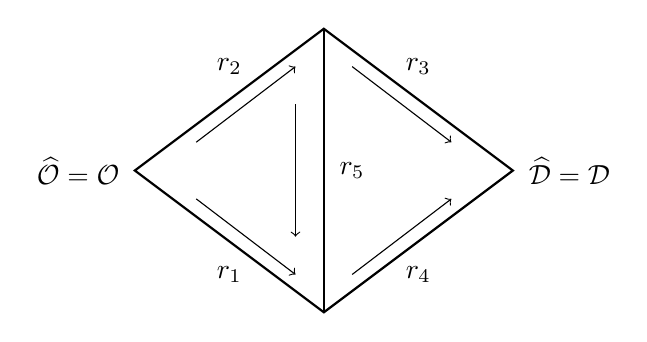
\begin{tikzpicture}[scale=1.2]

\coordinate (L) at (0,0);
\coordinate (T) at (2,1.5);
\coordinate (R) at (4,0);
\coordinate (B) at (2,-1.5);

\draw[thick] (L) -- (T) -- (R) -- (B) -- cycle;
\draw[thick] (T) -- (B);

\draw[->] (0.65,0.3) -- (1.7,1.1);

\draw[->] (0.65,-0.3) -- (1.7,-1.1);

\draw[->] (2.3,1.1) -- (3.35,0.3);

\draw[->] (2.3,-1.1) -- (3.35,-0.3);

\draw[->] (1.7, 0.7) -- (1.7, -0.7);

\node at (1,1.1) {$r_2$};
\node at (1,-1.1) {$r_1$};
\node at (3,1.1) {$r_3$};
\node at (3,-1.1) {$r_4$};
\node at (2.3, 0) {$r_5$};
\node at (-0.6, 0) {$\widehat{\mathcal{O}} = \widecheck{\mathcal{O}}$};
\node at (4.6, 0) {$\widehat{\mathcal{D}} = \widecheck{\mathcal{D}}$};
\end{tikzpicture}
\quad
\]
Analizziamo l'effetto della variazione del costo della strada $r_5$; passiamo da $\widehat{\tau_5}(\eta) = \widecheck{\tau_5}(\eta) = 0$ a 
$\widehat{\tau_5}(\eta) = \widecheck{\tau_5}(\eta) = 50$. Istanziamo dunque un nuovo \textbf{Parameters.py} (vedi \autoref{script:1} per specifica delle \textbf{@property}):
\begin{lstlisting}[style=myStile, caption={Parameters.py}, label={script:18}, escapeinside={(*@}{@*)}]
from typing import override

from utility.SafeArray import SafeArray #Vedi (*@\autoref{script:3}@*)
from utility.Operations import Operations #Vedi (*@\autoref{script:2}@*)
from utility.AbstractParam import AbstractParam

class Parameters(AbstractParam):

    @property
    def operation(self):
        return Operations.NASH_EQ_TIME_VARIATIONS
    
    @property
    def output_directory(self):
        #Directory di salvataggio dei dati uguale a quella di Parameters.py
        return "parameters\\parameters3" 
    
    @property
    def MIN(self) -> float:
        return 0.
    
    @property
    def MAX(self) -> float:
        return 50.
    
    @property
    def step(self) -> float:
        return 0.5
    
    @property
    def variation_hat(self) -> SafeArray:
        return SafeArray([0., 0., 0., 0., 1.])
    
    @property
    def variation_check(self) -> SafeArray:
        return SafeArray([0., 0., 0., 0., 1.])

    @property #(*@$\widehat{\Gamma}$@*)
    def Gamma_hat(self):
        return SafeArray([
            [0., 1., 0.],
            [1., 0., 1.],
            [1., 0., 0.],
            [0., 1., 1.],
            [0., 0., 1.]
        ])

    @property #(*@$\widecheck{\Gamma}$@*)
    def Gamma_check(self):
        return SafeArray([
            [0., 1., 0.],
            [1., 0., 1.],
            [1., 0., 0.],
            [0., 1., 1.],
            [0., 0., 1.]
        ])

    @override #(*@$\widehat{\tau}(\widehat{\eta}, \widecheck{\eta})$@*)
    def tau_hat(self, eta_hat, eta_check):
        return (
            SafeArray([
                45.,
                40. * eta_hat[1, 0],
                45.,
                40. * eta_hat[3, 0],
                0
            ])
        )

    @override #(*@$\widecheck{\tau}(\widehat{\eta}, \widecheck{\eta})$@*)
    def tau_check(self, eta_hat, eta_check):
        return (
            SafeArray([
                30.,
                20. * eta_check[1, 0] + 8. * eta_hat[1, 0],
                30.,
                20. * eta_check[1, 0] + 8. * eta_hat[1, 0],
                0
            ])
        )
\end{lstlisting}
Eseguendo il programma troviamo i seguenti grafici:
\begin{center}

\includegraphics[height=10cm]{../figures/Es1/grafico_main_costo.png}\\

\includegraphics[height=10cm]{../figures/Es1/grafico_hat_costo.png}

\includegraphics[height=10cm]{../figures/Es1/grafico_check_costo.png}
\end{center}
Con l'aumentare del costo della strada $r_5$ si ottiene un risultato inatteso: il tempo di attraversamento della rete diminuisce. Progressivamente
sempre più entità delle due popolazioni scelgono i percorsi che non contengono la strada $r_5$, finché nessuno la utilizza più, raggiungendo il minimo
del tempo di attraversamento. 

La rimozione di suddetta strada migliora la qualità del viaggio sulla rete: ci troviamo davanti a un caso di Paradosso di Braess \cite{BraessParadox}. 
Questa situazione è molto fragile: se esaminiamo il caso in cui $\widehat{\tau_5}(\eta) = \widecheck{\tau_5}(\eta) = 0$, facendo variare 
il numero di entità delle popolazioni, da $\widehat{\zeta} = \widecheck{\zeta} = 1$ a $\widehat{\zeta} = \widecheck{\zeta} = 3$:
\begin{lstlisting}[style=myStile, caption={Parameters.py}, label={script:19}, escapeinside={(*@}{@*)}]
from typing import override

from utility.SafeArray import SafeArray
from utility.Operations import Operations
from utility.AbstractParam import AbstractParam

class Parameters(AbstractParam):

    @property
    def operation(self):
        return Operations.NASH_EQ_POP_VARIATIONS
    
    @property
    def output_directory(self):
        return "parameters\\parameters3"
    
    @property
    def MIN(self) -> float:
        """
        La variazione parte da self.entity_number_hat (o check), definito come 1 se non sovrascritto.
        Vedi (*@\autoref{script:1}@*)
        """
        return 0.

    @property
    def MAX(self):
        """
        La variazione arriva aa self.entity_number_hat (o check), che vale 3 in questo caso
        Vedi (*@\autoref{script:1}@*)
        """
        return 2.
    
    @property
    def step(self) -> float:
        return 0.01

    @property
    def Gamma_hat(self):
        return SafeArray([
            [0., 1., 0.],
            [1., 0., 1.],
            [1., 0., 0.],
            [0., 1., 1.],
            [0., 0., 1.]
        ])

    @property
    def Gamma_check(self):
        return SafeArray([
            [0., 1., 0.],
            [1., 0., 1.],
            [1., 0., 0.],
            [0., 1., 1.],
            [0., 0., 1.]
        ])

    @override
    def tau_hat(self, eta_hat, eta_check):
        return (
            SafeArray([
                45.,
                40. * eta_hat[1, 0],
                45.,
                40. * eta_hat[3, 0],
                0
            ])
        )

    @override
    def tau_check(self, eta_hat, eta_check):
        return (
            SafeArray([
                30.,
                20. * eta_check[1, 0] + 8. * eta_hat[1, 0],
                30.,
                20. * eta_check[1, 0] + 8. * eta_hat[1, 0],
                0
            ])
        )
\end{lstlisting}
otteniamo:
\begin{center}

\includegraphics[height=10cm]{../figures/Es1/grafico_main_pop.png}\\

\includegraphics[height=10cm]{../figures/Es1/grafico_hat_pop.png}

\includegraphics[height=10cm]{../figures/Es1/grafico_check_pop.png}
\end{center}
Aumentando le entità delle due popolazioni si ottiene, a seguito di una breve crescita del tempo di attraversamento, una fase transitoria
costante, in cui le due popolazioni iniziano progressivamente ad utilizzare i due percorsi che non contengono $r_5$. Terminato il transitorio
costante nessuno utilizza $r_5$ e si perde il comportamento paradossale della rete: anche se la strada ha costo 0 non conviene
attraversarla.

\subsubsection{Esempio 2}
\label{subsubsec:Es2}

Introduciamo, sempre riprendendola da \cite[Cap. 3]{MR4911797}, la seguente rete:
\[
\quad
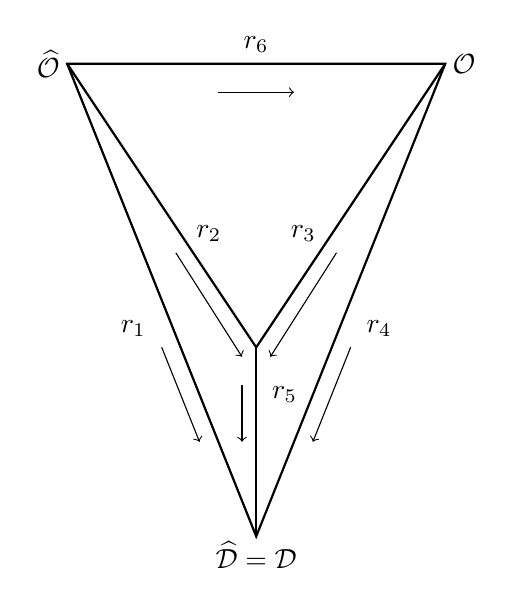
\begin{tikzpicture}[scale=1.2]

\coordinate (L) at (0,0);
\coordinate (R) at (4,0);
\coordinate (C) at (2,-3);
\coordinate (B) at (2,-5);


\draw[thick] (L) -- (R) -- (B) -- cycle;
\draw[thick] (L) -- (C);
\draw[thick] (R) -- (C);
\draw[thick] (C) -- (B);

\draw[->] (1.6,-0.3) -- (2.4,-0.3);

\draw[->] (1.15,-2) -- (1.85,-3.1);

\draw[->] (2.85,-2) -- (2.15,-3.1);

\draw[->] (1.85,-3.4) -- (1.85,-4);

\draw[->] (1, -3) -- (1.4, -4);

\draw[->] (3, -3) -- (2.6, -4);

\node at (0.7,-2.8) {$r_1$};
\node at (1.5,-1.8) {$r_2$};
\node at (2.5,-1.8) {$r_3$};
\node at (3.3,-2.8) {$r_4$};
\node at (2.3, -3.5) {$r_5$};
\node at (2, 0.2) {$r_6$};
\node at (-0.2, 0) {$\widehat{\mathcal{O}}$};
\node at (4.2, 0) {$\widecheck{\mathcal{O}}$};
\node at (2, -5.2) {$\widehat{\mathcal{D}} = \widecheck{\mathcal{D}}$};
\end{tikzpicture}
\quad
\]

Variando il costo della strada $r_6$ \textbf{solamente per la popolazione \textit{hat}}, da $\widehat{\tau_6}(\eta)=1$ a $\widehat{\tau_6}(\eta)=1.5$:
\begin{lstlisting}[style=myStile, caption={Parameters.py}, label={script:20}, escapeinside={(*@}{@*)}]
from typing import override

from utility.SafeArray import SafeArray
import numpy as np
from utility.Operations import Operations
from utility.AbstractParam import AbstractParam

class Parameters(AbstractParam):

    @property
    def operation(self):
        return Operations.NASH_EQ_TIME_VARIATIONS
    
    @property
    def output_directory(self) -> str:
        return "parameters\\parameters4"

    @property 
    def MIN(self):
        return 0.

    @property
    def MAX(self):
        return 0.5

    @property
    def step(self):
        return 0.01

    @property
    def Gamma_hat(self):
        return SafeArray([[1., 0., 0.],
                          [0., 1., 0.],
                          [0., 0., 0.],
                          [0., 0., 1.],
                          [0., 1., 0.],
                          [0., 0., 1.]])
    
    @property
    def Gamma_check(self) -> SafeArray:
        return SafeArray([[0., 0.],
                          [0., 0.],
                          [1., 0.],
                          [0., 1.],
                          [1., 0.],
                          [0., 0.]])
    
    @property
    def variation_hat(self):
        return SafeArray([0., 0., 0., 0., 0., 1.])
    
    @property
    def variation_check(self):
        return SafeArray([0., 0., 0., 0., 0., 0.])
    
    @override
    def tau_hat(self, eta_hat, eta_check):
        return (
            SafeArray([
                4.,
                1.+eta_hat[1, 0],
                np.inf,
                5.*eta_hat[3, 0]+5.*eta_check[3, 0],
                1.+eta_hat[4, 0]+eta_check[4, 0],
                1
            ])
        )
    
    @override
    def tau_check(self, eta_hat, eta_check):
        return (
            SafeArray([
                np.inf,
                np.inf,
                eta_check[2, 0],
                5.*eta_hat[3, 0]+5.*eta_check[3, 0],
                1.+eta_hat[4, 0]+eta_check[4, 0],
                np.inf
            ])
        )
\end{lstlisting}
otteniamo:
\begin{center}

\includegraphics[height=10cm]{../figures/Es2/grafico_main_costo.png}\\

\includegraphics[height=10cm]{../figures/Es2/grafico_hat_costo.png}

\includegraphics[height=5cm]{../figures/Es2/grafico_check_costo.png}
\end{center}
Come nella \autoref{subsubsec:Es1} osserviamo un Paradosso di Braess \cite{BraessParadox}. Questa volta, però, solo una delle due popolazioni
(\textit{check}) risente della variazione di costo di $r_6$, nonostante nessuna entità \textit{check} la attraversi: l'aggiunta di $r_6$, che
non migliora il tempo di attraversamento dell'unica popolazione che ne usufruisce (\textit{hat}), peggiora invece il tempo di attraversamento dell'altra.

Nuovamente si nota che questo stato paradossale è fragile: facendo variare, per esempio, il numero di entità nella popolazione \textit{check}, da $\widecheck{\zeta} = 1$
a $\widecheck{\zeta} = 6$:
\begin{lstlisting}[style=myStile, caption={Parameters.py}, label={script:21}, escapeinside={(*@}{@*)}]
from typing import override

from utility.SafeArray import SafeArray
import numpy as np
from utility.Operations import Operations
from utility.AbstractParam import AbstractParam

class Parameters(AbstractParam):

    @property
    def operation(self):
        return Operations.NASH_EQ_POP_VARIATIONS
    
    @property
    def output_directory(self) -> str:
        return "parameters\\parameters4"

    @property
    def MIN(self):
        """
        La variazione parte da self.entity_number_check, definito come 1 se non sovrascritto.
        Vedi (*@\autoref{script:1}@*)
        """
        return 0.

    @property
    def MAX(self):
        """
        La variazione arriva aa self.entity_number_check, che vale 6 in questo caso
        Vedi (*@\autoref{script:1}@*)
        """
        return 5.

    @property
    def step(self):
        return 0.05
    
    @property
    def variate_pop_hat(self) -> bool:
        return False
    
    @property
    def variate_pop_check(self) -> bool:
        return True

    @property
    def Gamma_hat(self):
        return SafeArray([[1., 0., 0.],
                          [0., 1., 0.],
                          [0., 0., 0.],
                          [0., 0., 1.],
                          [0., 1., 0.],
                          [0., 0., 1.]])
    
    @property
    def Gamma_check(self) -> SafeArray:
        return SafeArray([[0., 0.],
                          [0., 0.],
                          [1., 0.],
                          [0., 1.],
                          [1., 0.],
                          [0., 0.]])
    
    @override
    def tau_hat(self, eta_hat, eta_check):
        return (
            SafeArray([
                4.,
                1.+eta_hat[1, 0],
                np.inf,
                5.*eta_hat[3, 0]+5.*eta_check[3, 0],
                1.+eta_hat[4, 0]+eta_check[4, 0],
                1
            ])
        )
    
    @override
    def tau_check(self, eta_hat, eta_check):
        return (
            SafeArray([
                np.inf,
                np.inf,
                eta_check[2, 0],
                5.*eta_hat[3, 0]+5.*eta_check[3, 0],
                1.+eta_hat[4, 0]+eta_check[4, 0],
                np.inf
            ])
        )
\end{lstlisting}
risulta:
\begin{center}

\includegraphics[height=10cm]{../figures/Es2/grafico_main_pop.png}\\

\includegraphics[height=10cm]{../figures/Es2/grafico_hat_pop.png}

\includegraphics[height=5cm]{../figures/Es2/grafico_check_pop.png}
\end{center}
Durante un transitorio iniziale del tempo di percorrenza la popolazione \textit{hat} 
smette progressivamente di utilizzare la $r_6$ e, nonostante la popolazione \textit{check} aumenti, il suo tempo di percorrenza rimane costante:
viene perso il comportamento paradossale della rete.